\documentclass[final,onefignum,onetabnum]{siamart190516}

%% ------------------------------------------------------------------
%% Code used in examples, needed to reproduce 
%% ------------------------------------------------------------------
%% Used for \set, used in an example below
\usepackage{braket,amsfonts}

%% Used in table example below
\usepackage{array}

%% Used in table and figure examples below
\usepackage[caption=false]{subfig}
%% Used for papers with subtables created with the subfig package
\captionsetup[subtable]{position=bottom}
\captionsetup[table]{position=bottom}

%% Used for PgfPlots example, shown in the "Figures" section below.
\usepackage{pgfplots}

%% Used for creating new theorem and remark environments
\newsiamthm{claim}{Claim}
\newsiamremark{remark}{Remark}
\newsiamremark{hypothesis}{Hypothesis}
\crefname{hypothesis}{Hypothesis}{Hypotheses}

%% Algorithm style, could alternatively use algpseudocode
\usepackage{algorithmic}

%% For figures
\usepackage{graphicx,epstopdf}

%% For referencing line numbers
\Crefname{ALC@unique}{Line}{Lines}

%% For creating math operators
\usepackage{amsopn}
\DeclareMathOperator{\Range}{Range}

%% ------------------------------------------------------------------
%% Macros for in-document examples. These are not meant to reused for
%% SIAM journal papers.
%% ------------------------------------------------------------------
\usepackage{xspace}
\usepackage{bold-extra}
\usepackage[most]{tcolorbox}
\newcommand{\BibTeX}{{\scshape Bib}\TeX\xspace}
\newcounter{example}
\colorlet{texcscolor}{blue!50!black}
\colorlet{texemcolor}{red!70!black}
\colorlet{texpreamble}{red!70!black}
\colorlet{codebackground}{black!25!white!25}

\newcommand\bs{\symbol{'134}} % print backslash in typewriter OT1/T1
\newcommand{\preamble}[2][\small]{\textcolor{texpreamble}{#1\texttt{#2 \emph{\% <- Preamble}}}}

\lstdefinestyle{siamlatex}{%
  style=tcblatex,
  texcsstyle=*\color{texcscolor},
  texcsstyle=[2]\color{texemcolor},
  keywordstyle=[2]\color{texemcolor},
  moretexcs={cref,Cref,maketitle,mathcal,text,headers,email,url},
}

\tcbset{%
  colframe=black!75!white!75,
  coltitle=white,
  colback=codebackground, % bottom/left side
  colbacklower=white, % top/right side
  fonttitle=\bfseries,
  arc=0pt,outer arc=0pt,
  top=1pt,bottom=1pt,left=1mm,right=1mm,middle=1mm,boxsep=1mm,
  leftrule=0.3mm,rightrule=0.3mm,toprule=0.3mm,bottomrule=0.3mm,
  listing options={style=siamlatex}
}

\newtcblisting[use counter=example]{example}[2][]{%
  title={Example~\thetcbcounter: #2},#1}

\newtcbinputlisting[use counter=example]{\examplefile}[3][]{%
  title={Example~\thetcbcounter: #2},listing file={#3},#1}

\DeclareTotalTCBox{\code}{ v O{} }
{ %fontupper=\ttfamily\color{texemcolor},
  fontupper=\ttfamily\color{black},
  nobeforeafter,
  tcbox raise base,
  colback=codebackground,colframe=white,
  top=0pt,bottom=0pt,left=0mm,right=0mm,
  leftrule=0pt,rightrule=0pt,toprule=0mm,bottomrule=0mm,
  boxsep=0.5mm,
  #2}{#1}

% Stretch the pages
\patchcmd\newpage{\vfil}{}{}{}
\flushbottom

%% ------------------------------------------------------------------
%% End of macros for in-document examples. 
%% ------------------------------------------------------------------

%% ------------------------------------------------------------------
%% HEADING INFORMATION
%% ------------------------------------------------------------------
\begin{tcbverbatimwrite}{tmp_\jobname_header.tex}
\title{Guide to Using SIAM's \LaTeX\ Style\thanks{Submitted to the editors DATE.
\funding{Funding information goes here.}}}

\author{Dianne Doe\thanks{Imagination Corp., Chicago, IL (\email{ddoe@imag.com}).}
\and Paul T. Frank\thanks{Department of Applied Math, Fictional University, Boise, ID (\email{ptfrank@fictional.edu}, \email{jesmith@fictional.edu}).}
\and Jane E. Smith\footnotemark[3]}

% Custom SIAM macro to insert headers
\headers{Guide to Using  SIAM'S \LaTeX\ Style}{Dianne Doe, Paul T. Frank, and Jane E. Smith}
\end{tcbverbatimwrite}
\input{tmp_\jobname_header.tex}

% Optional: Set up PDF title and authors
\ifpdf
\hypersetup{ pdftitle={Guide to Using  SIAM'S \LaTeX\ Style} }
\fi

%% ------------------------------------------------------------------
%% END HEADING INFORMATION
%% ------------------------------------------------------------------

%% ------------------------------------------------------------------
%% MAIN Document
%% ------------------------------------------------------------------
\begin{document}
\maketitle

%% ------------------------------------------------------------------
%% ABSTRACT
%% ------------------------------------------------------------------
\begin{tcbverbatimwrite}{tmp_\jobname_abstract.tex}
\begin{abstract}
  Documentation is given for use of the SIAM standard \LaTeX\ and \BibTeX\
  macros.  Instructions and suggestions for compliance with SIAM style
  standards are also included. Familiarity with standard \LaTeX\ commands is assumed.
\end{abstract}

\begin{keywords}
  \LaTeX, \BibTeX, SIAM Journals, Documentation 
\end{keywords}

\begin{AMS}
  00A20 
\end{AMS}
\end{tcbverbatimwrite}
\input{tmp_\jobname_abstract.tex}
%% ------------------------------------------------------------------
%% END HEADER
%% ------------------------------------------------------------------

\section{Introduction}
\label{sec:intro}

This file is documentation for the SIAM \LaTeX\ style, including how
to typeset the main document, the \BibTeX\ file, and any supplementary
material. More information
about SIAM's editorial style can be found in the style manual, available
at \url{https://www.siam.org/journals/pdf/stylemanual.pdf}.
%
The major changes in the SIAM standard class are summarized in \cref{sec:changes}.
%
The SIAM \LaTeX\@ files can be found at
\url{https://www.siam.org/journals/auth-info.php}. The files that
are distributed for the standard macros are given below. 
\begin{itemize}
\item \texttt{siamart190516.cls} (required): Main SIAM standard \LaTeX\ class file.
\item \texttt{siamplain.bst} (required): Bibliographic style file for
  \BibTeX.
\item \texttt{docsiamart.tex}: Produces this documentation.
\item \texttt{references.bib}: \BibTeX\ database for this
  documentation and examples.
\item \texttt{ex\_article.tex}: Template for article.
\item \texttt{ex\_supplement.tex}: Template for supplement.
\item \texttt{ex\_shared.tex}: Template for shared information for
  article and supplement.
\end{itemize}
To use these files, put \texttt{siamart190516.cls} and
\texttt{siamplain.bst} in the directory with your
paper or, alternatively, into your \LaTeX\@ and \BibTeX\@ paths,
respectively. 
%
The outline of a SIAM \LaTeX\ article is shown in
\cref{ex:outline}. Templates are provided and discussed in more detail
in \cref{sec:template}.

\begin{example}[label={ex:outline},listing only,%
  listing options={style=siamlatex,{morekeywords=[1]{maketitle},
      morekeywords=[2]{siamart190516}},}]%
  {Document outline}
\documentclass{siamart190516}
% Preamble consisting of:
% Packages and macro definitions go here.
% Define title, authors, headers here.
\begin{document}
\maketitle
% Other front matter goes here: abstract, keywords, AMS subjects.
% Main body goes here.
% Appendices goes here (optional).
% Acknowledgements go here (optional).
% Bibliography goes here.
\end{document}
\end{example}

\section{Class options}
\label{sec:class-options}

Class options can be included in the bracketed argument of the
command, separated by commas. The possible class options are:
\begin{itemize}
\item \code{review} --- Recommended for submitting your manuscript to
  a SIAM journal.  Adds line numbers as well as the statement ``This
  manuscript is for review purposes only'' to the bottom of each page.
\item \code{final} --- Turns off the black boxes that help authors
  identify lines that are too long. The final published version will
  have this option on.
\item \code{supplement} --- Specifies that the file is a supplement
  and not the main document, causing changes in the appearance of the
  title and numbering; see \cref{sec:supplement} for details.
\item \code{hidelinks} --- Turns off colors on hyperlinks; see
  \cref{sec:cr+hyp}. The hyperlinks still exist, but there is no color
  to differentiate them.
  The final published version will have this option on.
\end{itemize}


\section{Front matter}
\label{sec:front}
The title and author parts are formatted using the standard
\code{\title}, \code{\author}, and \code{\maketitle} commands as
described in Lamport \cite{La86}. The title and author should be
declared in the preamble. The title and author names are automatically
converted to uppercase in the document.
%
If there is more than one author, each additional author should be preceded by
the \code{\and} command.  
%
The addresses and support acknowledgments are added via
\code{\thanks}. Each author's thanks should specify their address.
The support acknowledgment should be put in the title thanks,
unless specific support needs to be specified for individual authors,
in which case it should follow the author address.  
%
The header for this file was produced by the code in \cref{ex:header}, including an
example of a shared footnote. Each thanks produces a footnote, so the
footnote of the second author is \#3.
%
The command
\code{\headers{title}{authors}} command, with
the title (possibly shortened to fit) and the authors' names, creates
the page headers, automatically converted to uppercase.

\examplefile[label={ex:header},listing only,%
listing options={style=siamlatex,%
deletetexcs={and,thanks,title,author},%
{moretexcs=[2]{and,thanks,title,author,maketitle,headers,email}}}
]{Title and authors in preamble}{tmp_\jobname_header.tex}

\newpage
Following the author and title is the abstract, key words listing, and AMS subject
classifications, designated using the \code{abstract}, \code{keywords}, and \code{AMS}
environments. 
Authors are responsible for providing AMS numbers which can be found
on the AMS web site \cite{AMSMSC2010}. The abstract, keywords, and AMS subject classifications
for this document are specified in \cref{ex:abstract}.

\examplefile[label={ex:abstract},%
before upper={\preamble{\bs newcommand\{\bs BibTeX\}\{\{\bs scshape Bib\}\bs TeX\bs xspace\}}},
listing only,%
listing options={style=siamlatex,%
{morekeywords=[2]{abstract,keywords,AMS}}}
]{Abstract, keywords, and AMS classifications}{tmp_\jobname_abstract.tex}

A more complete example, including a PDF supplement, that uses the
included files \texttt{ex\_article.tex}, \texttt{ex\_supplement.tex},
and \texttt{ex\_shared.tex} is discussed in
\cref{sec:template}. The example files can be used as a starting point
for producing a document.

\section{Cross references and hyperlinks}
\label{sec:cr+hyp}

SIAM now supports cross references and hyperlinks via the
\texttt{cleveref} and \texttt{hyperef} packages, which are loaded by
the class file.

\subsection{Cleveref}
\label{sec:cleveref}

SIAM strongly recommends using the commands provided by 
the \texttt{cleveref} package for cross referencing.
The package is automatically loaded and already customized
to adhere to SIAM's style guidelines. 
%
To create a cross reference, use the command \code{\cref} (inside
sentence) or \code{\Cref} (beginning of a sentence) in place of the
object name and \code{\ref}. 
%
The \texttt{cleveref}
package enhances \LaTeX's cross-referencing features, allowing
the format of cross references to be determined automatically
according to the ``type" of cross reference (equation, section, etc.)
and the context in which the cross reference is used.
%
So, the package
\emph{automatically} inserts the object name as well as the
appropriate hyperlink; see \cref{ex:cref}.
It may require two \LaTeX\@ compilations for the references to show up
correctly.
Additional examples are shown in the sections below
for equations, tables, figures, sections, etc.

\begin{example}[label=ex:cref,bicolor,listing options={style=siamlatex,%
{morekeywords=[2]{cref,ref}}}]{Advantage of using cleveref}
The normal way to get a cross reference with a hyperlink requires a
lot of typing: \hyperref[thm:mvt]{Theorem~\ref*{thm:mvt}}.
The \texttt{cleveref} package gets both the name and hyperlink
automatically using a single macro: \cref{thm:mvt}.
It also handles multiple references with the same macro, such as
\cref{thm:mvt,fig:pgfplots,fig:testfig}.
\end{example}

%

%\newpage
\subsection{Hyperef}
\label{sec:hyperef}

Hyperlinks are created with the \code{\href} and \code{\url} commands,
as shown in \cref{ex:href}.
SIAM has also defined the \code{\email} command, as shown in
\cref{ex:header}.
You can hide links (i.e., turn off link colors) with the \code{hidelinks} option.

\begin{example}[label={ex:href},bicolor,%
listing options={style=siamlatex,%
{morekeywords=[2]{href,url}}}]{Creating hyperlinks}
The \href{https://www.siam.org}{SIAM homepage} has general information.
Note that the colored text will \emph{not} appear in the print version
nor will the hyperlink be active, so the writer may want to specify
the location explicitly instead by using \url{https://www.siam.org}.
\end{example}

Note that homepage links via \code{\url} in the \code{\thanks} environment require
special formatting for the tilde (\string~) character. The formatting
is used in the template and shown in \cref{ex:shared}.


\section{Math and equations}
\label{sec:math}
Here we show some example equations, with numbering, and examples of
referencing the equations. SIAM now includes the package 
\texttt{amsmath} by default, and we include some of its features as
well, although the reader should consult the package user manual for
further guidance \cite{amsmath,shortmath}.
 Several of the example are adapted 
from Mittlebach and Goossen's guide to \LaTeX~\cite{MiGo04}.

\Cref{ex:textmath} is a straightforward example of inline mathematics
equations that does not use any special packages or features.

\begin{example}[label={ex:textmath},bicolor]{Inline math}
The following shows an example of math in text: 
Let $S=[s_{ij}]$ ($1\leq i,j\leq n$) be a $(0,1,-1)$-matrix of order $n$.
\end{example}

In \cref{ex:bbm}, we show the recommended method for getting
blackboard fonts using the \texttt{amsfonts} package. This is not
loaded by default and must be included in the preamble.

\begin{example}[label={ex:bbm},bicolor,before upper={\preamble{\bs
      usepackage\{amsfonts\}}},%
listing options={style=siamlatex,%
{morekeywords=[2]{mathbb}}}]{Blackboard math}
Blackboard bold characters, such as $\mathbb{C}$ and $\mathbb{R}$,
should be created with the \texttt{amsfonts} package, although this
is not included by default.
\end{example}

%\newpage
\Cref{ex:smallmatrix} shows the \code{smallmatrix} environment for an
inline matrix from the \texttt{amsmath} package, which is included by
default.

\begin{example}[label={ex:smallmatrix},bicolor,%
listing options={style=siamlatex,%
{morekeywords=[2]{smallmatrix}}}]{Inline matrix}
Matrices of no more than two rows appearing in text can be created
as shown in the next example:
$B = \bigl[ \begin{smallmatrix} B_{11} & B_{12} \\ 
  B_{21} & B_{22} \end{smallmatrix} \bigr]$.
\end{example}

Bigger matrices can be rendered with environments from
the \texttt{amsmath} package, such as \code{bmatrix} and
\code{pmatrix} used in
\cref{ex:matrices}.

\begin{example}[label={ex:matrices},bicolor,%
listing options={style=siamlatex,%
{morekeywords=[2]{bmatrix,pmatrix}}}]{Creating matrices}
Display matrices can be rendered using environments from \texttt{amsmath}:
\begin{equation}\label{eq:matrices}
  S=\begin{bmatrix}1&0\\0&0\end{bmatrix}
  \quad\text{and}\quad
  C=\begin{pmatrix}1&1&0\\1&1&0\\0&0&0\end{pmatrix}.
\end{equation}
\Cref{eq:matrices} shows some example matrices.
\end{example}

\newpage
\Cref{ex:dmo} shows how to use the \code{\DeclareMathOperator} command
from the \texttt{amsopn} package to declare the \code{\Range} macro. 
(This example also uses the \texttt{braket} package for the
\code{\set} macro, but this is not necessarily recommended by SIAM.)
%
\begin{example}[label={ex:dmo},%
before upper={\preamble{\bs usepackage\{braket,amsfonts,amsopn\}}\\
\noindent\preamble{\bs DeclareMathOperator\{\bs Range\}\{Range\}}},%
bicolor,%
listing options={style=siamlatex,%
{moretexcs=[2]{Range}}}
]{Declaring math operators}
An example of a math operator:
\begin{equation}\label{eq:range}
  \Range(A) = \set{ y \in \mathbb{R}^n | y = Ax }.
\end{equation}
\end{example}

%\newpage
\Cref{ex:foo} shows how to use the \code{align} environment from
\texttt{amsmath} to easily align multiple equations.

\begin{example}[label={ex:foo},bicolor,%
listing options={style=siamlatex,%
{morekeywords=[2]{align}}}]{Aligned equations}
\Cref{eq:a,eq:b,eq:c} show three aligned equations.
\begin{align} 
  f &= g, \label{eq:a} \\
  f' &= g', \quad\text{and} \label{eq:b} \\
  \mathcal{L}f &= \mathcal{L}g \label{eq:c}.
\end{align}
\end{example}

Another way to number a set of equations is the
\code{subequations} environment from \texttt{amsmath}, as shown in \cref{ex:aligned}.

\begin{example}[label={ex:aligned},bicolor,%
listing options={style=siamlatex,%
{morekeywords=[2]{subequations}}}]{Subequations}
We calculate the Fr\'{e}chet derivative of $F$ as follows:
\begin{subequations}
\begin{align}
  F'(U,V)(H,K) 
  &= \langle R(U,V),H\Sigma V^{T} + U\Sigma K^{T} -
  P(H\Sigma V^{T} + U\Sigma K^{T})\rangle \label{eq:aa} \\
  &= \langle R(U,V),H\Sigma V^{T} + U\Sigma K^{T}\rangle 
  \nonumber \\
  &= \langle R(U,V)V\Sigma^{T},H\rangle + 
  \langle \Sigma^{T}U^{T}R(U,V),K^{T}\rangle. \label{eq:bb}
\end{align}
\end{subequations}
\Cref{eq:aa} is the first line, and \cref{eq:bb} is the last line.
\end{example}

%\newpage
~

For an equation split over multiple lines, \cref{ex:ml} shows the
usage of the \code{multline} environment provided by \texttt{amsmath}.

~

\begin{example}[label={ex:ml},bicolor,%
listing options={style=siamlatex,%
{morekeywords=[2]{multline}}}]{Equation split across lines}
We claim that the projection $g(U,V)$ is given by the pair of matrices:
\begin{multline} \label{eq:ml}
  g(U,V) = \biggl( \frac{R(U,V)V\Sigma^{T}U^{T} 
    - U\Sigma V^{T}R(U,V)^{T}}{2}U,\\
  \frac{R(U,V)^{T}U\Sigma V^{T}-V \Sigma^{T}U^{T}R(U,V)}{2}V \biggr).
\end{multline}
\end{example}

\section{Theorem-like environments}
\label{sec:thm}
SIAM loads \texttt{ntheorem} package and uses it to define the following
theorem-like environments:
\code{theorem}, 
\code{lemma}, 
\code{corollary},
\code{definition}, and
\code{proposition}.
SIAM also defines a \code{proof} environment that automatically
inserts the symbol ``$\,\proofbox\,$'' at the end of any proof, even if it ends in an
equation environment. \emph{Note that the document may need to be
  compiled twice for the mark to appear.}
Some of the calculus examples were adapted from \cite{CalcI}. 
%
% An example theorem and lemma declaration is shown in \cref{ex:theorem}.  These
% are all numbered in the same sequence and produce labels in small caps
% with an italic body. Use the command \code{\textup} to produce Roman
% type for numbers and parentheses.
%
\Cref{ex:theorem} shows usage of the \code{theorem} environment. 
An optional argument can be used to name the theorem.
\Cref{ex:cor} illustrates a corollary, without a name, and the
proof environment.

~

\begin{example}[label=ex:theorem,bicolor,parbox=false,%
listing options={style=siamlatex,%
{morekeywords=[2]{theorem}}}]{Theorem}
\begin{theorem}[Mean Value Theorem]\label{thm:mvt}
  Suppose $f$ is a function that is continuous on the closed interval
  $[a,b]$.  and differentiable on the open interval $(a,b)$.
  Then there exists a number $c$ such that $a < c < b$ and
  \begin{displaymath}
    f'(c) = \frac{f(b)-f(a)}{b-a}.
  \end{displaymath}
  In other words, $f(b)-f(a) = f'(c)(b-a)$.
\end{theorem}
\end{example}

\begin{example}[label=ex:cor,bicolor,parbox=false,%
listing options={style=siamlatex,%
{morekeywords=[2]{corollary,proof}}}]%
{Corollary and proof}
\begin{corollary}
  Let $f(x)$ be continuous and differentiable everywhere. If $f(x)$
  has at least two roots, then $f'(x)$ must have at least one root.
\end{corollary}
\begin{proof}
  Let $a$ and $b$ be two distinct roots of $f$.
  By \cref{thm:mvt}, there exists a number $c$ such that
  \begin{displaymath}
    f'(c) = \frac{f(b)-f(a)}{b-a} = \frac{0-0}{b-a} = 0.
  \end{displaymath}
\end{proof}
\end{example}

SIAM also defines commands to create your own theorem- and
remark-like environments:
\begin{itemize}
\item \code{newsiamthm} --- Small caps header, italized body. 
\item \code{newsiamremark} --- Italics header, roman body.
\end{itemize}
Each command takes two arguments. The first is the environment name,
and the second is the name to show in the document. These commands should
be used instead of \code{\newtheorem}.
\Cref{ex:claim,ex:ref} shows how to use the commands above, including how to
specify the plural version for \texttt{cleveref} if it is unusual.

\begin{example}[label=ex:claim,bicolor,%
before upper={\preamble{\bs newsiamthm\{claim\}\{Claim\}}\\
\noindent\preamble{\bs newsiamremark\{hypothesis\}\{Hypothesis\}}\\
\noindent\preamble{\bs crefname\{hypothesis\}\{Hypothesis\}\{Hypotheses\}}},%
parbox=false,%
listing options={style=siamlatex,%
{morekeywords=[2]{claim,proof,hypothesis}}}]{New theorem-like environment}
\begin{claim}\label{cl:constant}
  If $f'(x) = 0$ for all $x \in (a,b)$ then $f(x)$ is constant on $(a,b)$.
\end{claim}
\begin{hypothesis}\label{hyp1}
The function $f$ is continuously differentiable.
\end{hypothesis}
\begin{hypothesis}\label{hyp2}
The random variable is normally distributed.
\end{hypothesis}
\end{example}

% \begin{example}[label=ex:remark,bicolor,%
% before upper={\preamble{\bs newsiamremark\{expl\}\{Example\}}},%
% parbox=false,%
% listing options={style=siamlatex,%
% {morekeywords=[2]{expl}}}]{New remark-like environment}
% \begin{expl}[Trivial note]\label{ex:a}
%   Let $f(x) = 2$. Since $f'(x) = 0$ for all $x$, $f$ is constant
%   everywhere.
% \end{expl}
% \end{example}

\begin{example}[label=ex:ref,bicolor,listing options={style=siamlatex,%
{morekeywords=[2]{cref}}}]{References}
We can reference multiple types of objects with a single reference:
\cref{cl:constant,thm:mvt,hyp1,hyp2}.
\end{example}


\section{Tables}
\label{sec:tab}
Table captions should go above the tables.
\Cref{ex:simpletable} shows the code to generate a
\cref{tab:simpletable}.
A more complicated example is shown in 
\cref{ex:table}, which generates \cref{tab:KoMa14}. This
example uses subfloats via the \texttt{subfig} package, as well as
special column options from the \texttt{array} package.

\begin{tcbverbatimwrite}{tmp_\jobname_simpletable.tex}
\begin{table}[tbhp]
{\footnotesize
  \caption{Example table}\label{tab:simpletable}
\begin{center}
  \begin{tabular}{|c|c|c|} \hline
   Species & \bf Mean & \bf Std.~Dev. \\ \hline
    1 & 3.4 & 1.2 \\
    2 & 5.4 & 0.6 \\ \hline
  \end{tabular}
\end{center}
}
\end{table}
\end{tcbverbatimwrite}

\examplefile[label={ex:simpletable},%
listing only, listing options={style=siamlatex}]%
{Example table.}{tmp_\jobname_simpletable.tex}

\input{tmp_\jobname_simpletable.tex}

\begin{tcbverbatimwrite}{tmp_\jobname_table.tex}
\newcolumntype{R}{>{$}r<{$}}  %
\newcolumntype{V}[1]{>{[\;}*{#1}{R@{\;\;}}R<{\;]}} %
\begin{table}[tbhp]
{\footnotesize
 \captionsetup{position=top} %<- Needed for using subtables created with the subfig package 
  \caption{Example table adapted from Kolda and Mayo \rm{\cite{KoMa14}}.}\label{tab:KoMa14}
\begin{center}
  \subfloat[$\beta=1$]{
    \begin{tabular}{|r|R|V{3}|c|r@{\,$\pm$\,}l|} \hline
occ. & \multicolumn{1}{c|}{$\lambda$} & \multicolumn{4}{c|}{$\mathbf{x}$} & 
fevals &  \multicolumn{2}{c|}{time (sec.)}\\ \hline
 718 & 11.3476 &  0.5544 &  0.3155 &  1.2018 &  0.0977 &   45 & 0.17 & 0.06 \\ \hline 
 134 &  3.7394 &  0.2642 & -1.1056 &  0.2657 & -0.3160 &   31 & 0.12 & 0.05 \\ \hline 
   4 & \multicolumn{6}{c|}{\emph{--- Failed to converge ---}} & 0.21 & 0.10 \\ \hline 
 \end{tabular}}

  \subfloat[$\beta=-1$]{
    \begin{tabular}{|r|R|V{3}|c|r@{\,$\pm$\,}l|} \hline
occ. & \multicolumn{1}{c|}{$\lambda$} & \multicolumn{4}{c|}{$\mathbf{x}$} & 
fevals &  \multicolumn{2}{c|}{time (sec.)}\\ \hline
  72 & -1.1507 &  0.2291 &  0.6444 &  0.3540 & -0.8990 &   34 & 0.14 & 0.06 \\ \hline 
 624 & -6.3985 &  0.1003 &  0.1840 &  0.5305 &  1.2438 &   48 & 0.19 & 0.08 \\ \hline 
   2 & \multicolumn{6}{c|}{\emph{--- Failed to converge ---}} & 0.23 & 0.02 \\ \hline 
 \end{tabular}}
\end{center}
}
\end{table}
\end{tcbverbatimwrite}

\examplefile[label={ex:table},%
before upper={\preamble[\scriptsize]{\bs usepackage\{array\}}\\[-0.4em]
\noindent\preamble[\scriptsize]{\bs usepackage[caption=false]\{subfig\}}},%
listing only, listing options={%
  style=siamlatex,basicstyle=\ttfamily\scriptsize}]%
{Example table with subtables.}{tmp_\jobname_table.tex}

\input{tmp_\jobname_table.tex}

\section{Figures}
\label{sec:fig}

It is recommended that all figures be generated in high resolution.
In the past, SIAM has required encapsulated
postscript (EPS) format for final production. This is still an
acceptable format, but SIAM also now allows high-resolution 
PDF, JPEG, and PNG figures. 
%
If working with EPS images and using \texttt{pdflatex}, we
recommend the package \texttt{epstopdf} to automatically convert EPS
images to PDF for inclusion in PDF documents created by
\texttt{pdflatex}.
%
\Cref{ex:fig} shows the code to generate \cref{fig:testfig}.  This
example uses the \texttt{graphicx} package for the
\code{\includegraphics} command. 


\begin{tcbverbatimwrite}{tmp_\jobname_fig.tex}
\begin{figure}[tbhp]
  \centering
  \subfloat[$\epsilon_{\max}=5$]{\label{fig:a}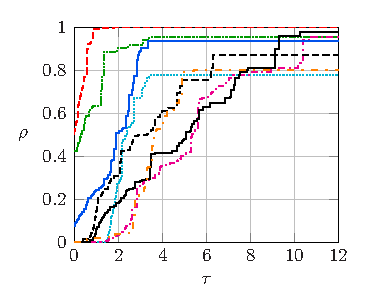
\includegraphics{lexample_fig1}}
  \subfloat[$\epsilon_{\max}=0.5$]{\label{fig:b}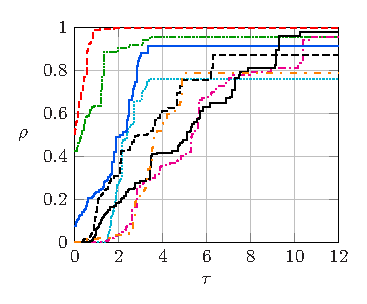
\includegraphics{lexample_fig2}}
  \caption{Example figure using external image files.}
  \label{fig:testfig}
\end{figure}
\end{tcbverbatimwrite}

\examplefile[label={ex:fig},%
before upper={\preamble[\scriptsize]{\bs usepackage\{graphicx,epstopdf\}}\\[-0.4em]
\noindent\preamble[\scriptsize]{\bs usepackage[caption=false]\{subfig\}}},%
listing only, listing options={%
  style=siamlatex,basicstyle=\ttfamily\scriptsize}]%
{Example figure with subfigures and external files}{tmp_\jobname_fig.tex}

\input{tmp_\jobname_fig.tex}

%\newpage
Another option for figures is a graphics-generator that is platform- and
format-independent.
PGF is a TeX macro package for generating  such graphics and works together with the most important TeX backend drivers, including pdftex and dvips. 
The user-friedly syntax layer called TikZ.
Here we show an example using \texttt{PGFPLOTS}, useful for drawing high-quality 
plots directly in \LaTeX.
\Cref{ex:data} and \cref{ex:pgfplots} shows the data and code, respectively, to generate \cref{fig:pgfplots}, adapted from \cite{pgfplots}.

\examplefile[label={ex:data},listing only,
listing options={style=siamlatex,basicstyle=\ttfamily\scriptsize}]%
{Example data file (data.dat)}{data.dat}

\begin{tcbverbatimwrite}{tmp_\jobname_tikz.tex}
\begin{figure}[tbhp]
  \centering
  \begin{tikzpicture}
    \begin{loglogaxis}[height=2.75in, grid=major,
      xlabel={Degrees of Freedom}, ylabel={$L_2$ Error},
      legend entries={$d=2$,$d=3$}]
      \addplot table [x=d2_dof,y=d2_l2_err] {data.dat};
      \addplot table [x=d3_dof,y=d3_l2_err] {data.dat};
    \end{loglogaxis}
  \end{tikzpicture}
  \caption{Example \texttt{PGFPLOTS} figure.}
  \label{fig:pgfplots}
\end{figure}
\end{tcbverbatimwrite}

\examplefile[label={ex:pgfplots},%
before upper={\preamble[\scriptsize]{\bs usepackage\{pgfplots\}}},%
listing only, listing options={%
  style=siamlatex}]%
{Example TikZ/PGF for platform-independent graphics.}{tmp_\jobname_tikz.tex}

\input{tmp_\jobname_tikz.tex}


%\newpage  
\section{Algorithms}
\label{sec:algs}

SIAM automatically includes the \texttt{algorithm} package in the
class definition. This provides the float environment.
Users have the choice of \texttt{algpseudocode},
\texttt{algorithmic}, and other packages for actually formatting the algorithm.
For example, \cref{alg:buildtree} is produced by the code in \cref{ex:alg}.
In order to reference lines within the algorithm, we need to tell the
\texttt{cleveref} package how to do the referencing, which is the
second line of \cref{ex:alg}. Then we can use the code
\code{\cref{line3}} to produce \cref{line3}.

\begin{tcbverbatimwrite}{tmp_\jobname_alg.tex}
\begin{algorithm}
\caption{Build tree}
\label{alg:buildtree}
\begin{algorithmic}[1]
\STATE{Define $P:=T:=\{ \{1\},\ldots,\{d\}$\}}
\WHILE{$\#P > 1$}
\STATE\label{line3}{Choose $C^\prime\in\mathcal{C}_p(P)$ with $C^\prime := \operatorname{argmin}_{C\in\mathcal{C}_p(P)} \varrho(C)$}
\STATE{Find an optimal partition tree $T_{C^\prime}$ }
\STATE{Update $P := (P{\setminus} C^\prime) \cup \{ \bigcup_{t\in C^\prime} t \}$}
\STATE{Update $T := T \cup \{ \bigcup_{t\in\tau} t : \tau\in T_{C^\prime}{\setminus} \mathcal{L}(T_{C^\prime})\}$}
\ENDWHILE
\RETURN $T$
\end{algorithmic}
\end{algorithm}
\end{tcbverbatimwrite}

\examplefile[float=htpb,label={ex:alg},%
before upper={\preamble[\scriptsize]{\bs usepackage\{algorithmic\}}\\[-0.4em]
\preamble[\scriptsize]{\bs Crefname\{ALC@unique\}\{Line\}\{Lines\}}},%
listing only, listing options={%
  style=siamlatex,basicstyle=\ttfamily\scriptsize}]%
{Example algorithm}{tmp_\jobname_alg.tex}

\input{tmp_\jobname_alg.tex}

\section{Sections}
\label{sec:sec}
Sections are denoted using standard \LaTeX\ section commands, i.e.,
\code{\section}, \code{\subsection}, etc. 
%
If you wish to end the section title with something other that a period (the default), you have to add the command \code{\nopunct} at the end of the title.

Appendices are created with the normal sectioning commands, following
the command \code{\appendix}. 
%
Titles of appendices created with
\code{\section} are preceded by the word ``Appendix,'' but not the
subsections or appendices created with \code{\section*}.
%
Unlike normal sections, appendix sections may be sensitive to blank lines
following the declaration, causing a new paragraph rather than the
text immediately following the appendix title. This can be corrected
by removing and blank lines.
%
Any numbered, labeled sections can be referenced using \code{\cref},
including those without a title.
%
Section titles are automatically inserted into the table of contents
and converted to bookmarks; see \cref{sec:spec-instr-pdf} for handling
special characters.


The acknowledgments section comes
immediately before the references and after any appendices. It should
be declared by \code{\section*{Acknowledgments}}.

%
% \Cref{ex:secref} shows how to reference sections.



% \begin{example}[label={ex:secref},lefthand ratio=0.4,bicolor,sidebyside,%
% listing options={style=siamlatex,basicstyle=\ttfamily\scriptsize,%
% deletetexcs={cref,Cref},{moretexcs=[2]{cref,Cref}}}]
% {Right and wrong ways to reference a section}
% Inside a sentence\dots\\
% Single: \cref{sec:intro}\\
% Range: \cref{sec:intro,sec:front,%
% sec:sec}\\
% Multiple: \cref{sec:intro,sec:sec,%
% sec:tab,sec:math,sec:thm}\\
% Appendix: \cref{sec:changes}\\

% Beginning of a sentence\dots\\
% Single: \Cref{sec:intro}\\
% Range: \Cref{sec:intro,sec:front,%
% sec:sec}\\
% Multiple: \Cref{sec:intro,sec:sec,%
% sec:tab,sec:math,sec:thm}\\
% Appendix: \Cref{sec:changes}\\


% Just don't do it this way\dots\\
% Section~\ref{sec:intro}  
% \end{example}

\section{Supplemental material}
\label{sec:supplement}

For several SIAM journals, authors are encouraged to submit
Supplementary Materials to complement their articles. This might
include additional figures or examples, animations, data sets used in
the paper, computer code used to generate figures or tables, or other
materials that are necessary to fully document the research contained
in the paper or to facilitate the readers' ability to understand and
extend the work.

\newpage
The class option \code{supplement} should be used in the
supplemental \LaTeX\ file provided for creating PDF supplemental material.
The supplement should have the same title and authors as the main
document.  The title is modified automatically by the SIAM
class file so that it is preceded by the text ``Supplementary
Materials'', followed by a colon.  
%
The numbering is modified so that
all sections, equations, figures, tables, algorithms, %
and so on to start with ``SM''. 
%
A supplement does have sections but does not have an
abstract, keywords, AMS classifications, or appendices.  The main
document and supplement can cross reference sections, equations,
theorem-like declarations, figures, tables, algorithms, etc.  However,
there is no sharing of references. The references are optional for a
supplement.
A template is provide, as discussed in \cref{sec:template}.

\section{Template}
\label{sec:template}

The files \texttt{ex\_article.tex}, \texttt{ex\_shared.tex},
and \texttt{ex\_supplement} \texttt{.tex} provide a template that can be used
for creating a \LaTeX\ document with an optional supplement.
%
\Cref{ex:artoutline,ex:suppoutline} give the outline of an article and
the supplement. In this case we
assume that the title and authors are defined in the
\texttt{ex\_shared.tex} file, shown in \cref{ex:shared}.
%
Cross referencing between the main document and the supplement is
enabled using the \texttt{xr-hyperref} package (included by the
SIAM class file). Use \code{\externaldocument}
to specify the external document to search for external
references.
%

\begin{example}[label={ex:artoutline},listing only,%
  listing options={style=siamlatex,%
    {morekeywords=[2]{externaldocument}}}]%
  {Document outline with supplement}
\documentclass{siamart190516}
% SIAM Shared Information Template
% This is information that is shared between the main document and any
% supplement. If no supplement is required, then this information can
% be included directly in the main document.


% Packages and macros go here
\usepackage{lipsum}
\usepackage{amsfonts}
\usepackage{graphicx}
\usepackage{epstopdf}
\usepackage{algorithmic}
\ifpdf
  \DeclareGraphicsExtensions{.eps,.pdf,.png,.jpg}
\else
  \DeclareGraphicsExtensions{.eps}
\fi

% Add a serial/Oxford comma by default.
\newcommand{\creflastconjunction}{, and~}

% Used for creating new theorem and remark environments
\newsiamremark{remark}{Remark}
\newsiamremark{hypothesis}{Hypothesis}
\crefname{hypothesis}{Hypothesis}{Hypotheses}
\newsiamthm{claim}{Claim}

% Sets running headers as well as PDF title and authors
\headers{An Example Article}{D. Doe, P. T. Frank, and J. E. Smith}

% Title. If the supplement option is on, then "Supplementary Material"
% is automatically inserted before the title.
\title{An Example Article\thanks{Submitted to the editors DATE.
\funding{This work was funded by the Fog Research Institute under contract no.~FRI-454.}}}

% Authors: full names plus addresses.
\author{Dianne Doe\thanks{Imagination Corp., Chicago, IL 
  (\email{ddoe@imag.com}, \url{http://www.imag.com/\string~ddoe/}).}
\and Paul T. Frank\thanks{Department of Applied Mathematics, Fictional University, Boise, ID 
  (\email{ptfrank@fictional.edu}, \email{jesmith@fictional.edu}).}
\and Jane E. Smith\footnotemark[3]}

\usepackage{amsopn}
\DeclareMathOperator{\diag}{diag}


%%% Local Variables: 
%%% mode:latex
%%% TeX-master: "ex_article"
%%% End: 

\externaldocument{ex_supplement}
\begin{document}
\maketitle
% Other front matter: abstract, keywords, subject classifications.
% Main body goes here.
% Appendices and/or acknowledgments.
% Bibliography
\end{document}
\end{example}

\begin{example}[label={ex:suppoutline},listing only,%
  listing options={style=siamlatex,%
    {morekeywords=[2]{supplement,siampretitle,externaldocument}}}]%
  {Supplement document outline}
\documentclass[supplement]{siamart190516}
% SIAM Shared Information Template
% This is information that is shared between the main document and any
% supplement. If no supplement is required, then this information can
% be included directly in the main document.


% Packages and macros go here
\usepackage{lipsum}
\usepackage{amsfonts}
\usepackage{graphicx}
\usepackage{epstopdf}
\usepackage{algorithmic}
\ifpdf
  \DeclareGraphicsExtensions{.eps,.pdf,.png,.jpg}
\else
  \DeclareGraphicsExtensions{.eps}
\fi

% Add a serial/Oxford comma by default.
\newcommand{\creflastconjunction}{, and~}

% Used for creating new theorem and remark environments
\newsiamremark{remark}{Remark}
\newsiamremark{hypothesis}{Hypothesis}
\crefname{hypothesis}{Hypothesis}{Hypotheses}
\newsiamthm{claim}{Claim}

% Sets running headers as well as PDF title and authors
\headers{An Example Article}{D. Doe, P. T. Frank, and J. E. Smith}

% Title. If the supplement option is on, then "Supplementary Material"
% is automatically inserted before the title.
\title{An Example Article\thanks{Submitted to the editors DATE.
\funding{This work was funded by the Fog Research Institute under contract no.~FRI-454.}}}

% Authors: full names plus addresses.
\author{Dianne Doe\thanks{Imagination Corp., Chicago, IL 
  (\email{ddoe@imag.com}, \url{http://www.imag.com/\string~ddoe/}).}
\and Paul T. Frank\thanks{Department of Applied Mathematics, Fictional University, Boise, ID 
  (\email{ptfrank@fictional.edu}, \email{jesmith@fictional.edu}).}
\and Jane E. Smith\footnotemark[3]}

\usepackage{amsopn}
\DeclareMathOperator{\diag}{diag}


%%% Local Variables: 
%%% mode:latex
%%% TeX-master: "ex_article"
%%% End: 

\externaldocument{ex_article}
\begin{document}
\maketitle
% No abstract, keywords, subject classifications.
% Main body goes here.
% No appendices or acknowledgments.
% Optional bibliography goes here.
\end{document}
\end{example}

%\newpage
\Cref{ex:shared} (from \texttt{ex\_shared.tex}) shows how the
``shared'' title and authors may be defined across the main document
and a supplement. 
%
Note the use of the \code{\string} command in the URL for the tilde;
this is only necessary inside the \code{\thanks} command.
%

\examplefile[label=ex:shared,listing only,%
listing options={style=siamlatex,firstline=19,lastline=40,%
{morekeywords=[2]{siampretitle,MakeUppercase,string}}}
]{Example of shared title and author macros}{ex_shared.tex}





\section{Bibliography}
\label{sec:bib}

The SIAM \BibTeX style file, now called \texttt{siamplain.bst}, has been updated to include the new keys listed below:
\begin{itemize}
\item \code{doi}: Digital object identifier, a unique alphanumeric string
\item \code{url}: Web address, usually impermanent
\item \code{urldate}: Date that the web address was last accessed
\item \code{eprint}: Archive identifier, a unique alphanumeric string
\item \code{eprintclass}: Archive class
\item \code{archive}: Archive URL, defaults to \nolinkurl{https://arXiv.org/abs}
\item \code{archivepreprint}: Archive name, defaults to ``arXiv''.
\item \code{eid}: Article ID, if there are no page numbers
\item \code{pagetotal}: Total number of pages, for use with article ID
\end{itemize}
Every entry type has been modified to include an optional link to a
DOI, a URL, and/or an archive preprint reference.
%
Additionally, the \code{article} entry now supports an Article ID,
\code{eid}, and number of pages, \code{pagetotal}.
%
To use this, include the following code in your \LaTeX\ source code:
\code{\bibliographystyle{siamplain}}.

\subsection{DOI}

A digital object identifier (DOI) is a unique alphanumeric string that provides a persistent link to its location on the Internet. The publisher assigns a DOI when your article is published and made available electronically. Using the \code{doi} field in \BibTeX to specify it, as shown for \cite{KoMa14} in \cref{ex:article}; observe the new \code{doi} field which produces a hyperlink in the citation.
Do not include the full URL, i.e., \nolinkurl{https://doi.org/} preceding the DOI.
Authors are highly advised to provide DOIs; if they are not provided, they
will be requested during the copyediting process. 

\examplefile[label=ex:article,listing only,%
listing options={style=siamlatex,firstline=1,lastline=12,{morekeywords=[2]{doi}}}
]{Example article in \BibTeX}{references.bib}

\subsection{URL}
There is also now support for the  \code{url} field. Generally, the DOI is preferred to the URL, since the DOIs should be permanent references. For that reason, it is good practice to specify the last date that the URL was accessed, which is specified by the optional \code{urldate} field. Reference \cite{Hi14} produced by \cref{ex:url} shows an example of using these fields.

\examplefile[label=ex:url,listing only,%
listing options={style=siamlatex,firstline=20,lastline=28,%
{morekeywords=[2]{url,urldate}}}
]{Example with the URL field in \BibTeX}{references.bib}

\subsection{Preprint servers such as arXiv}

More and more manuscripts are available on preprint servers. In fact,
SIAM's publication policy explicitly allows the final accepted version
of any article to be posted on a preprint server such as arXiv.

For an arXiv paper,
the \code{eprint} field is used to specify the identifier. The optional \code{eprintclass} field specifies the class. \Cref{ex:arxiv} shows the \BibTeX for \cite{PeKoPi14}. 

\examplefile[label=ex:arxiv,listing only,%
listing options={style=siamlatex,firstline=30,lastline=38,%
{morekeywords=[2]{eprint,eprintclass}}}
]{Example arXiv reference in \BibTeX}{references.bib}

\newpage
Other preprint servers are supported as well, but these require
specification of the fields \code{archive} and \code{archiveprefix}. In this case, the target URL is formed by concatenating the \code{archive}, a forward slash (\texttt{/}), and the \code{eprint}; and the text for the hyperlink is formed by concatenating the \code{archiveprevix}, a colon (:), and the \code{eprint}.
%
\Cref{ex:pubmed} shows the code to generate \cite{WoZhMeSh05}, including the preprint from PubMed.
Note that this example has both the journal citation as well as the link for the preprint.

\examplefile[label=ex:pubmed,listing only,%
listing options={style=siamlatex,firstline=40,lastline=55,%
{morekeywords=[2]{eprint,eprintclass,archive,archiveprefix}}}
]{Example PubMed reference in \BibTeX}{references.bib}

\subsection{Article ID}
Some journals use an article ID rather than page numbers. 
The field \texttt{eid} specifies the article ID. The optional field \texttt{pagetotal} can say the number
of pages in the document. An example of an article using these fields is shown in \cref{ex:eid} for citation \cite{Ne03}.

\examplefile[label=ex:eid,listing only,%
listing options={style=siamlatex,firstline=57,lastline=67,%
{morekeywords=[2]{eid,pagetotal}}}
]{Example article ID reference in \BibTeX}{references.bib}

\subsection{Software citations}

SIAM encourages software citations, both related technical publications as well as the software itself. A citation to a software package may look something like what is shown in \cref{ex:clawpack} for citation \cite{clawpack}. Notice the double braces around the \texttt{author} key; else, it would appear as ``C. D. Team''.

\examplefile[label=ex:clawpack,listing only,%
listing options={style=siamlatex,firstline=69,lastline=76,%
{morekeywords=[2]{key}}}
]{Example software reference in \BibTeX}{references.bib}

\appendix
\section{Summary of major changes}
\label{sec:changes}

Here we summarize the major changes in the latest version of
the SIAM standard \LaTeX\@ and \BibTeX\ classes:
\begin{itemize}
\item Change in file names: \texttt{siamart171218.cls} is replaced by
  \texttt{siamart190516.cls}, and the \texttt{siam.bst} bibliography style
  file is replaced by \texttt{siamplain.bst}; see \cref{sec:intro}.
\item Hyperlinking in cross references via the
  \texttt{cleveref} package, including customizations to adhere to
  SIAM conventions. Automatic PDF bookmarks enabled for sections,
  appendices, and references.
  See \cref{sec:cleveref}.
\item Colored hyperlinks (red for external, green for internal). Can
  be disabled with class options \code{hidelinks}; see \cref{sec:hyperef}.
\item New fields for \BibTeX, as listed in \cref{sec:bib}.
\item  Support for supplemental PDF files, including
  cross references between the supplement and the main document; see
  \cref{sec:supplement}. 
\item New command for setting headers: \code{\headings}; see
  \cref{sec:front}. 
\item Updated theorem-like and proof environments using
  \texttt{ntheorem} package; see \cref{sec:thm}.
\item Fixed handling of appendices to adhere to SIAM style guidelines;
  see \cref{sec:sec}.
\item Added \code{review} class option; see \cref{sec:class-options}.
\item Includes the following packages by default:
  \texttt{algorithm},
  \texttt{amsmath}, 
  \texttt{breakurl}, 
  \texttt{cleveref}, 
  \texttt{hypcap}, 
  \texttt{hyperef},
  \texttt{ifpdf},
  \texttt{ntheorem}, 
  \texttt{xcolor}, and
  \texttt{xr-hyperef}.
  Adds the \texttt{lineno}
  package if the \code{review} class option is enabled.
\end{itemize}

\section{Special modifications}

\subsection{Special macros}
In past versions, 
the SIAM standard \LaTeX\ class defined the following macros:
\code{\const},
\code{\diag},
\code{\grad},
\code{\Range},
\code{\rank}, and
\code{\supp}.
These are no longer declared; however, they can be redefined using the
\code{\DeclareMathOperator} command from the \texttt{amsopn}
package as demonstrated in \cref{ex:dmo}.

\subsection{Labeling objects sequentially}
SIAM recommends numbering objects by section number. 
However, if you prefer to number objects sequentially (e.g., Figure 5
would indicate the fifth figure appearing in the paper regardless of which section it is in), add the code from
\cref{ex:numbering} as documentclass options (e.g., \code{\documentclass[review,onefignum,onetabnum]{siamart190516}}).

\begin{example}[label=ex:numbering,listing only,%
listing options={style=siamlatex,{morekeywords=[2]{makeatletter,makeatother}},}]%
{Labeling objects sequentially}
oneeqnum % equations
onetabnum % tables
onefignum % figures
onealgnum % algorithms
onethmnum % theorem environments
\end{example}


\subsection{Appendices with no title}
The SIAM style manual \cite{siam} allows for an appendix that is
numbered (by a letter) but has no title. We have a special command to
create such an appendix: \code{\appendixnotitle}. This is equivalent
to a \code{\section} command in the appendix except that it has no
arguments.

\subsection{Changing the font of algorithm titles}
\label{sec:chang-font-algor}

Currently, the algorithm title font matches the figure and table title
fonts. To make the algorithm title font appear as small caps, insert
the code in \cref{ex:algfont} into the preamble.

\begin{example}[label=ex:algfont,listing only,%
listing options={style=siamlatex}]{Changing algorithm title font}
\makeatletter
\renewcommand{\ALG@name}{\sc Algorithm}
\makeatother
\end{example}

\subsection{Changing title of proof}
To change the title of a proof to, say, ``Proof of main theorem,''
simply use an optional argument as shown in
\cref{ex:newproof}.

\begin{example}[label=ex:newproof,listing only,%
listing options={style=siamlatex}]{Altered proof environment}
\begin{proof}[Proof of main theorem]
We now show ...
\end{proof}
\end{example}

\subsection{Special instructions for PDF bookmarks}
\label{sec:spec-instr-pdf}

Section titles are automatically inserted into the table of contents
and therefore used as PDF bookmarks. Some special symbols may not
correctly render. In that case, you can define alternate text as shown
in \cref{ex:specialtitle}, using the \code{\texorpdfstring} command
provided by the \texttt{hypertex} package. In this example, the
default bookmark would be ``Discussion of Z = X Y''; instead, it is
replaced by ``Discussion of Z = X union Y.''

\begin{example}[label=ex:specialtitle,listing only,%
listing options={style=siamlatex}]{PDF bookmarks for symbols in section titles}
\section{Discussion of \texorpdfstring{{\boldmath$Z=X \cup Y$}}{Z = X union Y}}
\end{example}


\bibliographystyle{siamplain}
\bibliography{references}

\end{document}
